\documentclass[twocolumn,prl,floatfix,superscriptaddress]{revtex4-2}
\usepackage{graphicx, subfigure, amsfonts, amssymb, amsmath, array, gensymb, fontenc, color, lipsum}
%\documentclass[aps,twocolumn,showpacs,preprintnumbers]{revtex4}
%\usepackage{graphicx}  % Include figure files
%\usepackage{subfigure}
%\usepackage{multirow}
%\linespread{1.0}
%\usepackage{fancyhdr}
%\usepackage{longtable}
%\usepackage{parskip}
%\usepackage[T1]{fontenc}
%\usepackage{dcolumn}
%\usepackage{bm}        
%\usepackage{amsfonts}  
%\usepackage{amsmath}   
%\usepackage{amssymb}
\usepackage{hyperref}
\hypersetup{colorlinks= true, allcolors=blue}
%\setcitestyle{aysep={}}
%\setlength{\parindent}{11pt}
\frenchspacing

\newcommand\partitle[1]{\textsc{#1}.}
\begin{document}

\title{On the reality of the quantum state once again}
\author{Gabriele Carcassi}
\affiliation{Physics Department, University of Michigan, Ann Arbor, MI 48109}
\author{Andrea Oldofredi}
\affiliation{Centre of Philosophy (CFUL), University of Lisbon, Portugal}
\author{Christine Aidala}
\affiliation{Physics Department, University of Michigan, Ann Arbor, MI 48109}
\vspace{2mm}

\date{\today}


\begin{abstract}
The ontological model framework introduced by Harrigan and Spekkens has been widely used to categorize quantum interpretations and as a basis for influential results such as the PBR theorem. In this paper we show that the model has a fundamental flaw: the epistemic structure it implicitly assumes does not follow the one dictated by quantum mechanics. Namely, the map between the epistemic states of the model and quantum density matrices is not even an order homomorphism in terms of the information entropy, consequently the epistemic content of mixed states is not mapped in a meaningful way. Moreover, by recasting the definitions of the model in terms of density matrices, we find that only $\psi$-epistemic interpretations are allowed by quantum mechanics, a result that is the opposite of the PBR theorem. We show that the cause of this mismatch is the effect of non-contextuality over mixed preparations that does not allow for a single decomposition of mixed states over pure states.
\end{abstract}

\maketitle

\section{Introduction}

%---e.g.\ standard Quantum Mechanics (QM) is classified as $\psi$-ontic and $\psi-$complete, hidden variable theories such as Bohm causal approach \cite{Bohm:1952aa} and Nelson mechanics \cite{Nelson:1966aa} are both considered $\psi$-ontic and $\psi$-incomplete, whereas Relational QM \cite{Rovelli:1996} and Quantum Bayesianism \cite{Fuchs:2002} are $\psi-$epistemic. 
%Since its publication HS paper has been subjected to several analyses and extensions as well as critical discussions showing some limitations of this approach (\cite{Leifer:2014, Leifer:2014b}, \cite{Leifer:2013}, \cite{Hermens:2021}, \cite{Wood:2015}, \cite{Ringbauer:2015}, \cite{Mazurek:2016}, \cite{Bartlett:2012}, \cite{Oldofredi:2020b}, \cite{Lewis:2012}, \cite{Ladyman:2021}). However, still today HS distinction is employed to argue what types of interpretations are possible. Referring to this, the PBR theorem \cite{PBR:2012}---a remarkable result derived on top of HS framework---rules out $\psi$-epistemic models. More precisely, PBR argued that in every model reproducing the statistics and predictions of QM the quantum state $\psi$ must represent real physical properties of the system under consideration---i.e.\ models must be $\psi-$ontic. Consequently, quantum theories cannot be $\psi-$epistemic. Given the importance of this claim and the resonance that such a theorem had (\cite{Renner:2012}, \cite{Hardy:2013}, \cite{Maroney:2014}, \cite{Patra:2013}, \cite{Mansfield:2016}, \cite{Schlosshauer:2012, Schlosshauer:2013, Schlosshauer:2014}, \cite{Ben:2017}, \cite{Rizzi:2018}, \cite{Oldofredi:2021}, \cite{DeBrota:2019}), it is worthwhile to look at HS framework again with more scrutiny in order to understand whether it is a technically sound starting point to draw conclusions on the nature of the quantum state.
 
In 2012 Pusey, Barrett and Rudolph published a formal result in \emph{Nature Physics}, widely known as the PBR theorem, showing that ``if the quantum state merely represents information about the real physical state of a system, then experimental predictions are obtained that contradict those of quantum theory'' (\cite{PBR:2012}, p.\ 475). Alternatively stated, PBR argued that in every model reproducing the statistics and predictions of Quantum Mechanics (QM) the quantum state $\psi$ must represent real physical properties of the system under consideration and not agents' knowledge---i.e.\ models must be $\psi-$ontic. Consequently, quantum theories cannot be $\psi-$epistemic. 

Such a theorem had a remarkable resonance (\cite{Leifer:2014, Leifer:2014b}, \cite{Renner:2012}, \cite{Colbeck:2017}, \cite{Hardy:2013}, \cite{Maroney:2014}, \cite{Patra:2013}, \cite{Mansfield:2016}, \cite{Schlosshauer:2012, Schlosshauer:2013, Schlosshauer:2014}, \cite{Aaronson:2013}), and questions about its actual meaning are still discussed today: on the one hand, it rules out interpretations of QM where $\psi$ merely represents information. On the other, scholars recently shown that non-trivial epistemic as well as statistical approaches to QM are not refuted by the PBR argument (\cite{Ben:2017}, \cite{Rizzi:2018}, \cite{Oldofredi:2021}, \cite{DeBrota:2019}).
	
In this essay we are not going to rebut the theorem itself. We instead aim to carefully re-examine one of its premises, i.e.\ Harrigan and Spekkens (HS) classification between $\psi-$ontic and $\psi-$epistemic ontological models  \cite{Harrigan:2010} on top of which the PBR result is derived. We believe that a careful examination of this assumption forces us to re-evaluate the significance of the PBR conclusion. 
		
HS proposed a rigorous classification in order to categorize the nature of the quantum state, i.e.\ to establish whether in a certain model $\psi$ corresponds to a real property of a quantum object, in that case the model is called $\psi-$ontic, or to some observer information, making it $\psi-$epistemic. While the original aim of this classification was to clarify Einstein's view of quantum theory, HS framework has been widely employed in the literature not only to categorize different interpretations, but also to argue what types of interpretations are admissible (\cite{Leifer:2013}, \cite{Leifer:2017}, \cite{Branciard:2014} \cite{Hermens:2021}, \cite{Wood:2015}, \cite{Ringbauer:2015}, \cite{Mazurek:2016}, \cite{Bartlett:2012}; cf.\ \cite{Oldofredi:2020b}, \cite{Lewis:2012}, \cite{Ladyman:2021} for critical discussions). Given the influence that HS framework and the PBR theorem have in the quantum foundations, it is worthwhile to look again at the former with more scrutiny in order to understand whether it is a sound basis to draw conclusions on the nature of the quantum state.

In this paper we will show two things:
\begin{enumerate}
	\item the information entropy as calculated on epistemic states does not match the one provided by quantum mechanics, meaning that the epistemic structures provided by QM and HS are incompatible;
	\item the density matrices associated with pure states overlap for non-orthogonal states (i.e. $\rho_\psi \rho_\phi \neq 0$), meaning that $\psi$-ontic models are ruled out, contrary to the PBR claim.
\end{enumerate}
Hence, our conclusion is that HS distinction is fundamentally flawed. The main problem lies in assuming that the epistemic state identifies a single probability distribution over the whole set of ontic states. We show that this, in essence, is an assumption of non-contextuality, which is also inherited by the PBR theorem, casting doubts on its validity.

\section{Summary of the Harrigan \& Spekkens Model}

We briefly review the main features of the classification provided by HS starting with the usual operational setting for QM. We have a preparation protocol $P$, which will be associated with a density operator $\rho$ on the relevant Hilbert space, and a measurement protocol $M$, represented by a POVM $\{ E_k\}$ where each $k$ represents a possible measurement outcome. The probability of obtaining a particular $k$ given a particular preparation $P$ and measurement $M$ is given by the generalized Born rule
\begin{equation}
	p(k|M, P)=\textrm{tr}(\rho E_k).
\end{equation}

An ontological model, as defined by HS, additionally assumes that there exists a set of states $\Lambda$, called \textbf{ontic states}, that provide the complete specification of the properties of a given physical object. A preparation $P$ will prepare a particular ontic state $\lambda$ according to the probability distribution $p(\lambda | P)$, which is referred to as \textbf{epistemic state}. The measurement outcome will depend only on the ontic state with probability $p(k|\lambda, M)$ (\cite{Harrigan:2010}, p.\ 128). This leads to the following expression:
\begin{equation}
	\int_\Lambda d\lambda p(k|\lambda, M) p(\lambda| P)= \textrm{tr}(\rho E_k).
\end{equation}
It is also assumed that a mixture of pure states $\{ \psi_i \}$ with probabilities $\{ w_i \}$ will be represented by
\begin{equation}\label{epistemic_mixing}
	\sum_i  w_i p(\lambda| P_{\psi_i}).
\end{equation}
As the epistemic states for mixed preparations are simply linear combinations of epistemic states for pure preparations, we can concentrate on the latter.

To classify an ontological model, we look at the relationship between quantum and ontic states. There are two broad categories. In a \textbf{$\psi$-ontic} model the wave function is a physical property of the ontic state, in the sense that given an ontic state $\lambda$ there is only one pure state preparation $P_\psi$ that could have prepared $\lambda$. As we can see in figure \ref{overlap}, this happens if the probability distributions do not overlap, i.e.\ if we have
\begin{equation}\label{ontic_condition}
	p(\lambda | P_{\psi})p(\lambda|P_{\phi})=0
\end{equation}
for all pairs of states $\psi$ and $\phi$. If a model is not $\psi$-ontic, then it is \textbf{$\psi$-epistemic}. In this case, $\lambda$ can be described by more than one quantum state and the wave function is taken to represent knowledge about the state preparation---in such models quantum states generate overlapping probability distributions over $\Lambda$ as shown in figure \ref{overlap} (b). A $\psi$-ontic model is said \textbf{$\psi$-complete} if the quantum states and the ontic states coincide. More precisely if 
\begin{equation}\label{complete_condition}
	p(\lambda|P_\psi)=\delta(\lambda-\lambda_{\psi}).
\end{equation}
All other models are \textbf{$\psi$-incomplete}.

To make this classification more concrete, let us give an example from classical mechanics. Consider the case where we prepare a particle according to a specific value of energy. The energy partitions phase space into mutually exclusive regions, and therefore we can understand the energy of the preparation as a property of the particle itself. According to HS, this would be an \emph{ontic property}. Consider now the case where we prepare a particle according to a specific temperature. When we take the particle from the oven, we are sampling from a Boltzmann distribution over different energies. However, unlike energy, temperature does not partition phase space because the same particle state could have been prepared by ovens at different temperature. Temperature is a property of the preparation and therefore an \emph{epistemic property}. 

%While the original aim of this classification was to clarify Einstein's view of quantum theory, it has been used in the literature to classify different interpretations (e.g. hidden variable theories such as Bohm pilot-wave theory \cite{Bohm:1952aa} and Nelson mechanics \cite{Nelson:1966aa} are both considered $\psi$-ontic and $\psi$-incomplete) and also to argue what types of interpretations are possible. Most notably, the PBR theorem \cite{PBR:2012} rules out any $\psi$-epistemic model. More precisely, PBR argued that in every model reproducing the statistics and predictions of Quantum Mechanics (QM) the quantum state $\psi$ must represent real physical properties of the system under consideration and not agents' knowledge---i.e.\ models must be $\psi-$ontic. Consequently, quantum theories cannot be $\psi-$epistemic.(TODO beef up this paragraph with citations). It is therefore worthwhile to look at the ontological model itself with more scrutiny.

\begin{figure}
\includegraphics[scale=.7]{ontic}
\caption{\footnotesize{Harrigan and Spekkens distinction between $\psi-$ontic (a) and $\psi-$epistemic (b) ontological models.}}\label{overlap}
\end{figure}

\section{Epistemic structure}

Let us consider more closely the space of epistemic states given by $p(\lambda | P)$ and equation \ref{epistemic_mixing}. To make the discussion more concrete, we assume to have a $\psi$-complete model of a single qubit representing the direction of spin.

Suppose we have a protocol that prepares either $z^+$ or $z^-$ with equal chance. This results in an epistemic state with equal distribution on $z^+$ and $z^-$. Similarly, suppose we have another protocol that prepares $x^+$ and $x^-$ with equal chance generating an epistemic state with equal distribution on $x^+$ and $x^-$. Note that such epistemic distributions do not overlap. Therefore, according to HS categorization, these correspond to two ontologically distinct states, making the preparation axis an ontological property of the system, regardless of the orientation. However, the respective density matrices would not just overlap: they would be the same maximally mixed state. Hence there seems to be a mismatch between the type of epistemic knowledge one can express in QM through mixed states and the type of epistemic knowledge described in the HS model. This needs to be investigated further.

Let us first characterize the extent of the discrepancy. In HS, the space of epistemic states $E_{HS}$ is the set of probability distributions over pure states, which is an infinite dimensional space. This is a direct consequence of defining the epistemic states as a distribution $p(\lambda|P)$ that, for each preparation $P$, assigns a well defined probability to each ontological state $\lambda$ \footnote{We will follow the convention of not distinguishing between probability and probability density.}. In QM, mixed states $E_{Q}$ are in one-to-one correspondence with the interior of the Bloch sphere, a three dimensional manifold. Looking at the difference in dimension, the discrepancy is not minor.

Note that the space of pure states $\Lambda$ is the same in both cases, one state for each direction of spin. Also note that all epistemic states in both spaces can be reached by mixture of pure states. The difference is that, in the quantum case, we have an ``aliasing'': different mixtures will give the same mixed states. Since each classical probability distribution corresponds to a unique mixing of pure states, we have a map $\iota : E_{HS} \mapsto E_{Q}$ that allows us to go from HS-epistemic states to density matrices, the Q-epistemic states. This map is surjective but not injective. Therefore $E_{Q}$ can be seen as a set of equivalence classes of $E_{HS}$. The key question, then, is the following: is the map $\iota$ sufficiently well behaved that we can understand the epistemic content of $E_{Q}$ based on the epistemic content of $E_{HS}$? Or is it so ill behaved that there is no connection between the two?

Ideally, one would like to say that $E_{HS}$ represents all possible epistemic states that include the knowledge about preparation, while $E_{Q}$ represents only those distinguishable through measurement. For example, one may want to say that the axis of preparation is, in principle, an ontologically distinct property, but this is not experimentally distinguishable. Therefore, distinct HS-epistemic states for each direction are projected by $\iota$ onto the same Q-epistemic state of maximum uncertainty. This sounds very plausible and appealing, but it turns out this is not the case. To show this fact we will concentrate on a single aspect of the map: how information entropy transforms under $\iota$. While there are other problems, we do not need to explore them: given the crucial role of entropy in information theory, its breakdown is sufficient to show that the epistemic structures of $E_{HS}$ and $E_{Q}$ are different.

Guided by figure \ref{fig_map}, let us study the map $\iota$ by going through a few examples. Since every pure state in quantum mechanics has zero entropy, we will require the same for all pure states in $E_{HS}$. Let us consider the HS-epistemic states specified by three uniform distributions over the Bloch sphere with support given by:
\begin{description}
	\item[A] the poles, $z^+$ and $z^-$;
	\item[B] the equator, all states on the x/y planes;
	\item[C] the whole sphere, all points.
\end{description}
Since we want the entropy for a single pure state to be zero, the entropy for case \textbf{A} will be 1 (uniform distribution between two discrete cases). Since $\iota(A)$ will be the maximally mixed state, this also corresponds to entropy 1. So far so good: $\iota$ maps entropy 1 to entropy 1! However, note that \textbf{A} is a measure zero set of \textbf{B}, which is a measure zero set of \textbf{C}. The entropy of \textbf{C} is therefore infinite with respect to \textbf{B} which is infinite with respect to \textbf{A}. On the other hand, \textbf{A}, \textbf{B} and \textbf{C} will all correspond to the same maximally mixed state, therefore $\iota$ collapses together epistemic states at different levels of infinity. Note that, in this case, $\iota$ picks the minimum entropy between the equivalent epistemic states. This is inconsistent with the idea that $E_{Q}$ represents states where knowledge is lost: that would pick the maximum possible entropy.

\begin{figure}
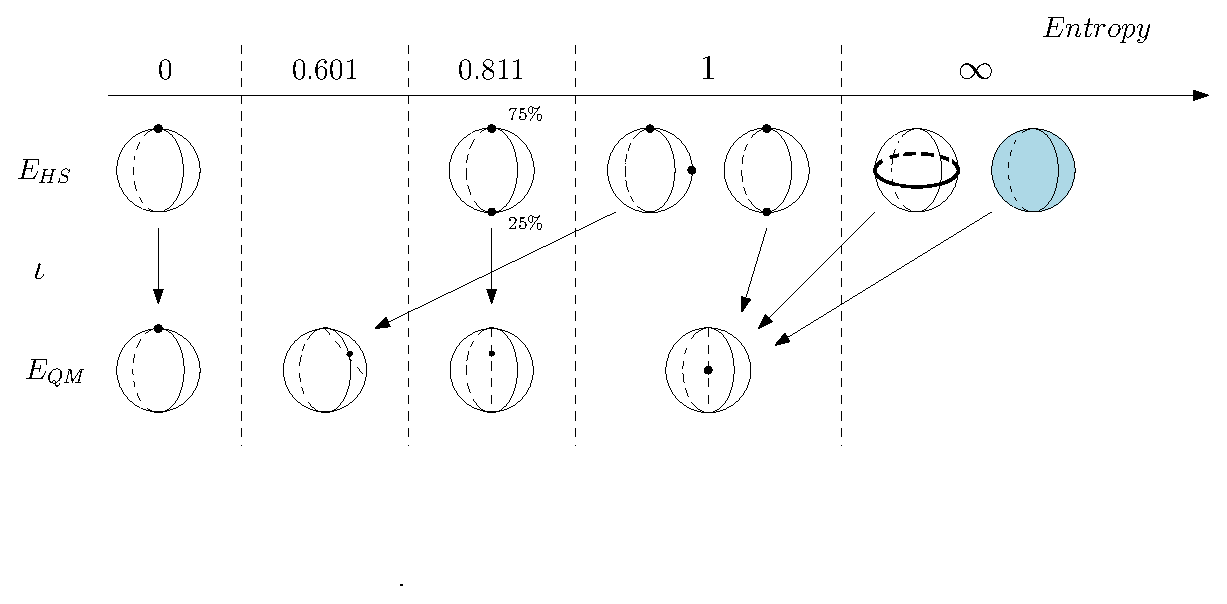
\includegraphics[scale=.4]{fig2}
\caption{\footnotesize{}}\label{fig_map}
\end{figure}

Now consider another uniform distribution over the support:
\begin{description}
	\item[D] the north pole and a point on the equator, $z^+$ and $x^+$.
\end{description}
This is yet another uniform distribution between two discrete cases, therefore in $E_{HS}$ the entropy is 1. However, $\iota(D)$ is not the maximally mixed state and therefore the entropy is less than 1. This means that epistemic states that are isoentropic in $E_{HS}$ are not isoentropic in $E_{Q}$. If we think as $E_{HS}$ and $E_{Q}$ as partially ordered by information entropy, then $\iota$ is not an order preserving map. Therefore, the epistemic structures represented by $E_{HS}$ and $E_{Q}$ are not isomorphic.

The seemingly innocuous assumption that $p(\lambda|P)$ is well defined for all preparations $P$ and for all states $\lambda$ imposes a classical probability space which follows the rules of classical information theory, and prevents the state space $\Lambda$ from supporting an epistemic structure compatible with quantum theory. 

This suggests an obvious follow up: what if we start by assuming that the set of pure states $\Lambda$ supports the correct epistemic structure, the one associated with density matrices, and use the same definitions of $\psi$-ontic and $\psi$-epistemic? We can rephrase condition \ref{ontic_condition} directly in terms of density matrices as $\rho_1 \rho_2 = 0$ which, for pure states, becomes:
\begin{equation}
	|\psi_1\rangle\langle\psi_1|\psi_2\rangle\langle\psi_2| = 0.
\end{equation}
That is, two pure states are non-overlapping if and only if $\langle\psi_1|\psi_2\rangle=0$, i.e. if they are orthogonal. Alternatively, we could ask that the probability of being in the support of the second given the first be zero. For pure states, we get $\langle\psi_2|\psi_1\rangle\langle\psi_1|\psi_2\rangle = 0$, which leads to the same condition. Or we could define the overlap in terms of the entropy of the mixture and still find the same result.

However we look at it, we reach the following result:
\begin{align}\label{conclusion}
	\parbox{2.8in}{Non-orthogonal pure quantum states overlap and are therefore epistemic.}
\end{align}
This should not be surprising: even in classical probability two distributions are non-overlapping if and only if they are orthogonal with respect to the inner product $\int \rho_1 \rho_2 d\lambda$.

Therefore, we have the following result: if we want a set of pure states that is able to support the epistemic structure of QM, they must be ``overlapping'' and thus we must have a $\psi$-epistemic model. This may seem in contradiction with the PBR theorem. Nonetheless, we believe that there is no contradiction, since there is no model in the HS classification that is compatible with quantum theory. In other words, the categorization itself is flawed.

\section{Discussion}

Let us now ask a crucial question: Why does assuming that $p(\lambda|P)$ is well defined lead to an epistemic structure incompatible with QM?

It is widely understood that one feature of quantum theory is contextuality: a measurement cannot be conceived as revealing pre-existing values. We may be tempted to think that we have one context before and one after the measurement. This does not work because we have a related dual effect on preparations. In the same way that we cannot understand quantum measurements as selecting from a single joint probability distribution for all properties, we cannot understand quantum preparations as constructing a single joint probability distribution over all properties. To fully understand how this works, let us review how probability spaces behave in both classical and quantum mechanics.

A ``classical'' probability space is made of three objects: a sample space $\Omega$ representing all possible cases (e.g.\ all points in phase-space for a classical system); a $\sigma$-algebra $\Sigma_\Omega$ over $\Omega$  representing all statements of interest (e.g.\ ``the position is between 2 and 3 meters''); a measure $\mu : \Sigma_\Omega \to \mathbb{R}$ associating each statement with a probability. Note how we have a single probability distribution over the whole space.

In QM we start with a similar structure: a set of states $\mathcal{H}$ representing all possible cases (i.e.\ the Hilbert space) and a $\sigma$-algebra $\Sigma_{\mathcal{H}}$ representing all statements of interest. This is where the similarity ends. To specify a mixed state---a ``quantum distribution''---we use a density matrix $\rho : \mathcal{H} \to \mathcal{H}$. To get a probability distribution, we need to specify an observable $O$. The observable $O$ identifies an orthogonal basis and we take the sub-algebra $\Sigma_O \subset \Sigma_{\mathcal{H}}$ defined on those states. We can then associate $\Sigma_O$ with a measure $\mu_O : \Sigma_O \to \mathbb{R}$, which is therefore not on the whole space $\Sigma_{\mathcal{H}}$.

Mathematically, what we call context is a $\sigma$-algebra: a set of propositions upon which we assign probabilities. This fact explains why we cannot simply use classical rules in QM. Classical mechanics has only one context, so we can always mix and match statements however we please. In QM, propositions about different observables live in different $\sigma$-algebras---in different probability spaces---and therefore cannot be combined.

One may think that we can get away by assuming that, at each time, there is a ``true'' context. And this seems to work in some cases. Given any density matrix $\rho$, there exists a (non-unique) privileged context: this is the one in which we can express $\rho = \sum p_i |\psi_i \rangle \langle \psi_i|$ as the mix of orthogonal pure states. If $\rho$ is itself a pure state, any basis that includes it will be a privileged context. This privileged context provides us the probability distribution over which the information entropy is calculated. After a measurement, the privileged context changes to one that includes the eigenstates of the chosen observable. However, this does not work in general.

Suppose to consider two density matrices $\rho_1$ and $\rho_2$ with different eigenstates and then to create the mixture $\rho = p_1 \rho_1 + p_2 \rho_2$. The context of the mixture will not be the same as the original contexts. It will, in fact, even depend on $p_1$, $p_2$. That is, when mixing preparations we are not simply combining two probability distributions over the same context, like in classical mechanics, but we are combining the contexts themselves to create a new one. Contextuality not only affects measurements, but, dually, preparations as well. And this affects how information entropy is calculated and the overall epistemic structure.

To sum up, assuming that $p(\lambda|P)$ exists means assuming that there is a single probability space, a single $\sigma$-algebra, a single set of propositions to which all probabilities are assigned. This is exactly assuming non-contextuality. While this can be made to work for pure state-to-pure state transitions during measurements, mixing preparations leads to an epistemic structure that is fundamentally non-contextual, leading to inconsistencies with quantum information. To allow for contextuality we should assume that for each observable $O$ we have a probability $p_O(\lambda_O|P)$ of having prepared one of the eigenstates, such that $\sum_{\lambda_O} p_O(\lambda_O|P) = 1$. While we have a single state space $\Lambda$, we do not have a single probability space over the whole space. The entropy of the preparation would be the lowest entropy across all contexts.


\section{Conclusion}

%Number of words for the conclusion: 159

%\bibliographystyle{ieeetr}
\bibliography{PhDthesis}


\end{document}